\subsection{RQ2a: retraining fixes the shortcut almost anywhere}
\label{sec:fix}
Retraining one block of the full fine-tuned model for one epoch on clean data removes the shortcut, whichever block is
chosen. Block~0 removes \retrainRemovedBZeroFullFT{} of the gap and block~1 \retrainRemovedBOneFullFT, although the
name's effect only reaches the answer position in blocks 9--11; every single block passes the removal criterion in all
seeds. The location matters a little when the budget is small: after only 100 steps, retraining the late blocks
\{9, 10, 11\} removes more of the gap than retraining the early blocks \{0, 2, 4\} in every seed, by
\budgetLateMinusEarlyFullFT. We had predicted an advantage of at least 0.20, which held only in seed 0.

\subsection{Why any block works: the counter-examples}
\label{sec:counterexample-ablation}
The clean-twin data used for retraining still contains the name sentence, with each name on both positive and negative
reviews. These counter-examples could teach any block that the names carry no label information. We repeated the
retraining with the name sentence removed from the clean data, all other settings matched (Fig.~\ref{fig:nonames}).
For full fine-tuning, block~0 then removes \ccNoNamesBZeroFullFT{} of the gap instead of \ccWithNamesBZeroFullFT, and
the same collapse happens for every block: all \ccCountedBlocksFullFT{} single blocks that remove the shortcut with the
names fail without them in at least two seeds. The pattern is the same for LoRA rank 64 (\ccCountedBlocksLoraRSixtyFour{} of
\ccPassWithNamesLoraRSixtyFour{} blocks) and rank 4 (\ccCountedBlocksLoraRFour{} of \ccPassWithNamesLoraRFour). For
retraining, \emph{what} the model sees decides the outcome; \emph{where} it is retrained does not. This is the shortcut
counterpart of the observation by Hase et al.~\cite{hase2023localization} for factual edits, with a causal explanation
of why the location does not matter here.

\begin{figure}[t]
\centering
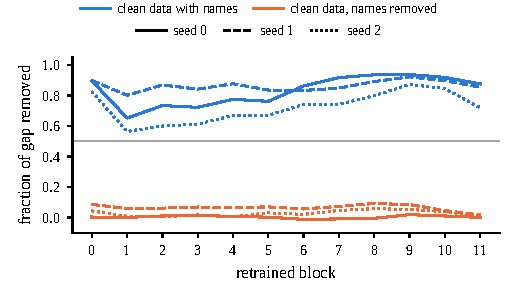
\includegraphics[width=\columnwidth]{figures/paper/fig_g_nonames.pdf}
\caption{Retraining one block of the full fine-tuned shortcut model on clean data with the name sentence (the
counter-examples) and with it removed. The horizontal line is the removal threshold.}
\label{fig:nonames}
\end{figure}

\subsection{RQ3a: does finding predict retraining?}
Across the 12 single blocks, the fraction removed by swapping and by retraining is rank-correlated for full fine-tuning
(Spearman \spearmanSwapRetrainFullFT). The \emph{ranking} of blocks agrees, but the \emph{set} of blocks that work does
not: swaps single out blocks 9--11, whereas retraining works everywhere. With the counter-example ablation, the location
found by the tools does not tell us where retraining must happen.
